
% This LaTeX was auto-generated from MATLAB code.
% To make changes, update the MATLAB code and republish this document.

\documentclass{article}
\usepackage{graphicx}
\usepackage{color}

\sloppy
\definecolor{lightgray}{gray}{0.5}
\setlength{\parindent}{0pt}

\begin{document}

    
    
\section*{MATLAB programming course for beginners, supported by Wagatsuma Lab@Kyutech}

\begin{par}
/* The MIT License (MIT): Copyright (c) 2021 Hiroaki Wagatsuma and Wagatsuma Lab@Kyutech
\end{par} \vspace{1em}
\begin{par}
Permission is hereby granted, free of charge, to any person obtaining a copy of this software and associated documentation files (the "Software"), to deal in the Software without restriction, including without limitation the rights to use, copy, modify, merge, publish, distribute, sublicense, and/or sell copies of the Software, and to permit persons to whom the Software is furnished to do so, subject to the following conditions:
\end{par} \vspace{1em}
\begin{par}
The above copyright notice and this permission notice shall be included in all copies or substantial portions of the Software.
\end{par} \vspace{1em}
\begin{par}
THE SOFTWARE IS PROVIDED "AS IS", WITHOUT WARRANTY OF ANY KIND, EXPRESS OR IMPLIED, INCLUDING BUT NOT LIMITED TO THE WARRANTIES OF MERCHANTABILITY, FITNESS FOR A PARTICULAR PURPOSE AND NONINFRINGEMENT. IN NO EVENT SHALL THE AUTHORS OR COPYRIGHT HOLDERS BE LIABLE FOR ANY CLAIM, DAMAGES OR OTHER LIABILITY, WHETHER IN AN ACTION OF CONTRACT, TORT OR OTHERWISE, ARISING FROM, OUT OF OR IN CONNECTION WITH THE SOFTWARE OR THE USE OR OTHER DEALINGS IN THE SOFTWARE. */
\end{par} \vspace{1em}

\subsection*{Contents}

\begin{itemize}
\setlength{\itemsep}{-1ex}
   \item Specifications and requirements
   \item Main program
\end{itemize}


\subsection*{Specifications and requirements}

\begin{enumerate}
\setlength{\itemsep}{-1ex}
   \item @Time    : 2021-1-16
   \item @Author  : Hiroaki Wagatsuma
   \item @Site    : https://github.com/hirowgit/1B0\_matla\_optmization\_course
   \item @IDE     : MATLAB R2018a
   \item @File    : A3\_Objects\_and\_Path\_Plus.m
\end{enumerate}


\subsection*{Main program}

\begin{par}
clear all
\end{par} \vspace{1em}
\begin{verbatim}
clc

A1_ExcelRead_and_Plot_Normal;

contr=[-0.15,0.15,0.7,0.7,-0.7,-0.7,-0.15,-0.15,0.15,0.15;1,1,1,-1,-1,1,1,-1,-1,1];
gAng=@(x1,y1,x2,y2) atan2(y2-y1,x2-x1);
RotM=@(theta) [cos(theta),-sin(theta);sin(theta),cos(theta)];

% Pcontr=RotM(gAng(x1,y1,x2,y2))*contr+repmat([x1;y1],[1,size(contr,2)]);


% ~~~~~~~~~MakeQTMovie <initialize> (start)~~~~~~~~~~~~~~
% You need to place "MakeQTMovie.m" (c) Copyright Malcolm Slaney, Interval Research, March 1999.
% in the same folder of this file

Flag_write_Movie=1;
Nm=1; % the serial number of the movie
f_folder='movie'; % the output folder of the movie
if ~isdir(f_folder); mkdir(f_folder); end
f_prefix='outputMoviePathM_c_'; % the output file name
if Flag_write_Movie == 1
    MovieFileName = strcat(f_prefix,num2str(Nm),'.mov');
    fprintf('Creating the movie file %s.\n', fullfile(f_folder,MovieFileName));
    MakeQTMovie('start',fullfile(f_folder,MovieFileName));
    MakeQTMovie('size', [480 360]);
    MakeQTMovie('quality', 1.0);
%     fps = 10;
  fps = 30;
end
% ~~~~~~~~~MakeQTMovie (end)~~~~~~~~~~~~~~

xRange=[50 200];
yRange=[50 200];
cmap1=colormap('Lines');

figure(4); clf
Dlen=[];
for i=1:Lsize
    sTraj_full=lineD2{i};
    Dlen(i)=length(sTraj_full);
    pp0{i}=plot(sTraj_full(:,1),sTraj_full(:,2),'.-','lineWidth',2,'MarkerSize',20); hold on;
%     pp0{i}=plot(sTraj_full(:,1),sTraj_full(:,2),'k-'); hold on;
    axis equal; grid on; xlabel('x'); ylabel('y');
    grid on;
    title(['Object movements in the trajectory ']);

    xx=1:size(contr,2);
    pp1{i}=plot(xx,xx,'Color',cmap1(i,:),'lineWidth',2);
%     set(pp{i},'erasemode','xor');

    set(gca,'xlim',xRange,'ylim',yRange);
end
Dlim=min(Dlen);

for k=1:Dlim-1

    for i=1:Lsize
        sTraj_full=lineD2{i};
        x1=sTraj_full(k,1); y1=sTraj_full(k,2);
        x2=sTraj_full(k+1,1); y2=sTraj_full(k+1,2);
        Pcontr=RotM(gAng(x1,y1,x2,y2))*contr+repmat([x1;y1],[1,size(contr,2)]);

        set(pp1{i},'XData',Pcontr(1,:),'YData',Pcontr(2,:));
%         plot(Pcontr(1,:),Pcontr(2,:),'.-','lineWidth',2,'MarkerSize',20),hold on;


        % ~~~~~~~~~MakeQTMovie <add a frame> (start)~~~~~~~~~~~~~~
        if Flag_write_Movie == 1
            MakeQTMovie('addfigure');
        end
        % ~~~~~~~~~MakeQTMovie (end)~~~~~~~~~~~~~~

    %     pause(0.2);
    %     drawnow;
%         hold off
    end
end

% ~~~~~~~~~MakeQTMovie  <finalize> (start)~~~~~~~~~~~~~~
if Flag_write_Movie == 1
    MakeQTMovie('framerate', fps);
    MakeQTMovie('finish');
    strMessage=sprintf('Please find the generated mov file in the folder "%s" as filename "%s"',f_folder,MovieFileName);
    disp(strMessage);
end
% ~~~~~~~~~MakeQTMovie (end)~~~~~~~~~~~~~~




% ~~~~~~~~~MakeQTMovie <comment>~~~~~~~~~~~~~~
% The generated mov file is recommended to open QuickTime Player 7 in the first place and resave a new mov file by the player.
% The new mov file generated by the player can be opened with a recent version of the QuickTime Player.

% ~~~~~~~~~MakeQTMovie (end)~~~~~~~~~~~~~~
\end{verbatim}

        \color{lightgray} \begin{verbatim}
ans = 

  struct with fields:

             Description: ''
                UserData: []
          DimensionNames: {'Row'  'Variables'}
           VariableNames: {1�~9 cell}
    VariableDescriptions: {}
           VariableUnits: {}
      VariableContinuity: []
                RowNames: {}


ans =

   202     9


varnames =

  1�~9 cell array

  Columns 1 through 7

    {'Var1'}    {'x1'}    {'y1'}    {'x2'}    {'y2'}    {'x3'}    {'y3'}

  Columns 8 through 9

    {'x4'}    {'y4'}


x1 =

   72.0000
   72.0000
   72.0000
   73.0141
   74.0282
   75.0423
   76.0563
   77.0704
   78.0845
   79.0986
   80.1127
   81.1268
   82.1408
   83.1549
   84.1690
   85.1831
   86.1972
   87.2113
   88.2254
   89.2394
   90.2535
   91.2676
   92.2817
   93.2958
   94.3099
   95.3239
   96.3380
   97.3521
   98.3662
   99.3803
  100.3944
  101.4085
  102.4225
  103.4366
  104.4507
  105.4648
  106.4789
  107.4930
  108.5070
  109.5211
  110.5352
  111.5493
  112.5634
  113.5775
  114.5915
  115.6056
  116.6197
  117.6338
  118.6479
  119.6620
  120.6761
  121.6901
  122.7042
  123.7183
  124.7324
  125.7465
  126.7606
  127.7746
  128.7887
  129.8028
  130.8169
  131.8310
  132.8451
  133.8592
  134.8732
  135.8873
  136.9014
  137.9155
  138.9296
  139.9437
  140.9577
  141.9718
  142.9859
  144.0000
  144.0000
  144.0727
  144.2853
  144.6296
  145.0974
  145.6804
  146.3704
  147.1591
  148.0384
  149.0000
  150.0357
  151.1372
  152.2963
  153.5048
  154.7545
  156.0370
  157.3443
  158.6680
  160.0000
  161.3320
  162.6557
  163.9630
  165.2455
  166.4952
  167.7037
  168.8628
  169.9643
  171.0000
  171.0000
  171.9634
  172.8555
  173.6790
  174.4367
  175.1312
  175.7654
  176.3420
  176.8637
  177.3333
  177.7535
  178.1271
  178.4568
  178.7453
  178.9954
  179.2099
  179.3914
  179.5428
  179.6667
  179.7659
  179.8432
  179.9012
  179.9428
  179.9707
  179.9877
  179.9963
  179.9995
  180.0000
  180.0000
  180.0000
  180.0000
  180.0000
  180.0000
  180.0000
  180.0000
  180.0000
  180.0000
  180.0000
  180.0000
  180.0000
  180.0000
  180.0000
  180.0000
  180.0000
  180.0000
  180.0000
  180.0000
  180.0000
  180.0000
  180.0000
  180.0000
  180.0000
  180.0000
  180.0000
  180.0000
  180.0000
  180.0000
  180.0000
  180.0000
  180.0000
  180.0000
  180.0000
  180.0000
  180.0000
  180.0000
  180.0000
  180.0000
  180.0000
  180.0000
  180.0000
  180.0000
  180.0000
  180.0000
  180.0000
  180.0000
  180.0000
  180.0000
  180.0000
  180.0000
  180.0000
  180.0000
  180.0000
  180.0000
  180.0000
  180.0000
  180.0000
  180.0000
  180.0000
  180.0000
  180.0000
  180.0000
  180.0000
  180.0000
  180.0000
  180.0000
  180.0000
  180.0000
  180.0000
  180.0000
  180.0000


y1 =

   54.0000
   54.0000
   54.0000
   54.0000
   54.0000
   54.0000
   54.0000
   54.0000
   54.0000
   54.0000
   54.0000
   54.0000
   54.0000
   54.0000
   54.0000
   54.0000
   54.0000
   54.0000
   54.0000
   54.0000
   54.0000
   54.0000
   54.0000
   54.0000
   54.0000
   54.0000
   54.0000
   54.0000
   54.0000
   54.0000
   54.0000
   54.0000
   54.0000
   54.0000
   54.0000
   54.0000
   54.0000
   54.0000
   54.0000
   54.0000
   54.0000
   54.0000
   54.0000
   54.0000
   54.0000
   54.0000
   54.0000
   54.0000
   54.0000
   54.0000
   54.0000
   54.0000
   54.0000
   54.0000
   54.0000
   54.0000
   54.0000
   54.0000
   54.0000
   54.0000
   54.0000
   54.0000
   54.0000
   54.0000
   54.0000
   54.0000
   54.0000
   54.0000
   54.0000
   54.0000
   54.0000
   54.0000
   54.0000
   54.0000
   54.0000
   54.0005
   54.0037
   54.0123
   54.0293
   54.0572
   54.0988
   54.1568
   54.2341
   54.3333
   54.4572
   54.6086
   54.7901
   55.0046
   55.2547
   55.5432
   55.8729
   56.2465
   56.6667
   57.1363
   57.6580
   58.2346
   58.8688
   59.5633
   60.3210
   61.1445
   62.0366
   63.0000
   63.0000
   64.0357
   65.1372
   66.2963
   67.5048
   68.7545
   70.0370
   71.3443
   72.6680
   74.0000
   75.3320
   76.6557
   77.9630
   79.2455
   80.4952
   81.7037
   82.8628
   83.9643
   85.0000
   85.9616
   86.8409
   87.6296
   88.3196
   88.9026
   89.3704
   89.7147
   89.9273
   90.0000
   90.0000
   91.0141
   92.0282
   93.0423
   94.0563
   95.0704
   96.0845
   97.0986
   98.1127
   99.1268
  100.1408
  101.1549
  102.1690
  103.1831
  104.1972
  105.2113
  106.2254
  107.2394
  108.2535
  109.2676
  110.2817
  111.2958
  112.3099
  113.3239
  114.3380
  115.3521
  116.3662
  117.3803
  118.3944
  119.4085
  120.4225
  121.4366
  122.4507
  123.4648
  124.4789
  125.4930
  126.5070
  127.5211
  128.5352
  129.5493
  130.5634
  131.5775
  132.5915
  133.6056
  134.6197
  135.6338
  136.6479
  137.6620
  138.6761
  139.6901
  140.7042
  141.7183
  142.7324
  143.7465
  144.7606
  145.7746
  146.7887
  147.8028
  148.8169
  149.8310
  150.8451
  151.8592
  152.8732
  153.8873
  154.9014
  155.9155
  156.9296
  157.9437
  158.9577
  159.9718
  160.9859
  162.0000


lineD =

  1�~1 cell array

    {202�~1 double}


lineD =

  1�~1 cell array

    {202�~2 double}


x2 =

   72.0000
   72.0000
   72.0000
   73.0141
   74.0282
   75.0423
   76.0563
   77.0704
   78.0845
   79.0986
   80.1127
   81.1268
   82.1408
   83.1549
   84.1690
   85.1831
   86.1972
   87.2113
   88.2254
   89.2394
   90.2535
   91.2676
   92.2817
   93.2958
   94.3099
   95.3239
   96.3380
   97.3521
   98.3662
   99.3803
  100.3944
  101.4085
  102.4225
  103.4366
  104.4507
  105.4648
  106.4789
  107.4930
  108.5070
  109.5211
  110.5352
  111.5493
  112.5634
  113.5775
  114.5915
  115.6056
  116.6197
  117.6338
  118.6479
  119.6620
  120.6761
  121.6901
  122.7042
  123.7183
  124.7324
  125.7465
  126.7606
  127.7746
  128.7887
  129.8028
  130.8169
  131.8310
  132.8451
  133.8592
  134.8732
  135.8873
  136.9014
  137.9155
  138.9296
  139.9437
  140.9577
  141.9718
  142.9859
  144.0000
  144.0000
  144.0916
  144.3590
  144.7914
  145.3776
  146.1067
  146.9676
  147.9495
  149.0413
  150.2320
  151.5107
  152.8663
  154.2878
  155.7643
  157.2848
  158.8382
  160.4136
  162.0000
  162.0000
  163.1243
  164.2448
  165.3574
  166.4583
  167.5436
  168.6094
  169.6517
  170.6667
  171.6504
  172.5990
  173.5085
  174.3750
  175.1947
  175.9635
  176.6777
  177.3333
  177.9264
  178.4531
  178.9095
  179.2917
  179.5957
  179.8177
  179.9538
  180.0000
         0
         0
         0
         0
         0
         0
         0
         0
         0
         0
         0
         0
         0
         0
         0
         0
         0
         0
         0
         0
         0
         0
         0
         0
         0
         0
         0
         0
         0
         0
         0
         0
         0
         0
         0
         0
         0
         0
         0
         0
         0
         0
         0
         0
         0
         0
         0
         0
         0
         0
         0
         0
         0
         0
         0
         0
         0
         0
         0
         0
         0
         0
         0
         0
         0
         0
         0
         0
         0
         0
         0
         0
         0
         0
         0
         0
         0
         0
         0
         0
         0
         0
         0
         0
         0


y2 =

   72.0000
   72.0000
   72.0000
   72.0000
   72.0000
   72.0000
   72.0000
   72.0000
   72.0000
   72.0000
   72.0000
   72.0000
   72.0000
   72.0000
   72.0000
   72.0000
   72.0000
   72.0000
   72.0000
   72.0000
   72.0000
   72.0000
   72.0000
   72.0000
   72.0000
   72.0000
   72.0000
   72.0000
   72.0000
   72.0000
   72.0000
   72.0000
   72.0000
   72.0000
   72.0000
   72.0000
   72.0000
   72.0000
   72.0000
   72.0000
   72.0000
   72.0000
   72.0000
   72.0000
   72.0000
   72.0000
   72.0000
   72.0000
   72.0000
   72.0000
   72.0000
   72.0000
   72.0000
   72.0000
   72.0000
   72.0000
   72.0000
   72.0000
   72.0000
   72.0000
   72.0000
   72.0000
   72.0000
   72.0000
   72.0000
   72.0000
   72.0000
   72.0000
   72.0000
   72.0000
   72.0000
   72.0000
   72.0000
   72.0000
   72.0000
   72.0000
   72.0000
   72.0000
   72.0000
   72.0000
   72.0000
   72.0000
   72.0000
   72.0000
   72.0000
   72.0000
   72.0000
   72.0000
   72.0000
   72.0000
   72.0000
   72.0000
   72.0000
   72.0911
   72.3542
   72.7734
   73.3333
   74.0182
   74.8125
   75.7005
   76.6667
   77.6953
   78.7708
   79.8776
   81.0000
   82.1224
   83.2292
   84.3047
   85.3333
   86.2995
   87.1875
   87.9818
   88.6667
   89.2266
   89.6458
   89.9089
   90.0000
         0
         0
         0
         0
         0
         0
         0
         0
         0
         0
         0
         0
         0
         0
         0
         0
         0
         0
         0
         0
         0
         0
         0
         0
         0
         0
         0
         0
         0
         0
         0
         0
         0
         0
         0
         0
         0
         0
         0
         0
         0
         0
         0
         0
         0
         0
         0
         0
         0
         0
         0
         0
         0
         0
         0
         0
         0
         0
         0
         0
         0
         0
         0
         0
         0
         0
         0
         0
         0
         0
         0
         0
         0
         0
         0
         0
         0
         0
         0
         0
         0
         0
         0
         0
         0


lineD =

  1�~2 cell array

    {202�~2 double}    {202�~1 double}


lineD =

  1�~2 cell array

    {202�~2 double}    {202�~2 double}


x3 =

  180.0000
  180.0000
  180.0000
  179.9722
  179.8900
  179.7553
  179.5698
  179.3354
  179.0538
  178.7269
  178.3566
  177.9445
  177.4925
  177.0025
  176.4763
  175.9155
  175.3222
  174.6981
  174.0449
  173.3646
  172.6589
  171.9296
  171.1785
  170.4076
  169.6185
  168.8131
  167.9932
  167.1606
  166.3171
  165.4645
  164.6047
  163.7395
  162.8707
  162.0000
  162.0000
  160.5803
  159.1684
  157.7723
  156.3998
  155.0588
  153.7571
  152.5027
  151.3034
  150.1671
  149.1016
  148.1149
  147.2148
  146.4091
  145.7058
  145.1127
  144.6377
  144.2887
  144.0735
  144.0000
  144.0000
  142.9859
  141.9718
  140.9577
  139.9437
  138.9296
  137.9155
  136.9014
  135.8873
  134.8732
  133.8592
  132.8451
  131.8310
  130.8169
  129.8028
  128.7887
  127.7746
  126.7606
  125.7465
  124.7324
  123.7183
  122.7042
  121.6901
  120.6761
  119.6620
  118.6479
  117.6338
  116.6197
  115.6056
  114.5915
  113.5775
  112.5634
  111.5493
  110.5352
  109.5211
  108.5070
  107.4930
  106.4789
  105.4648
  104.4507
  103.4366
  102.4225
  101.4085
  100.3944
   99.3803
   98.3662
   97.3521
   96.3380
   95.3239
   94.3099
   93.2958
   92.2817
   91.2676
   90.2535
   89.2394
   88.2254
   87.2113
   86.1972
   85.1831
   84.1690
   83.1549
   82.1408
   81.1268
   80.1127
   79.0986
   78.0845
   77.0704
   76.0563
   75.0423
   74.0282
   73.0141
   72.0000
         0
         0
         0
         0
         0
         0
         0
         0
         0
         0
         0
         0
         0
         0
         0
         0
         0
         0
         0
         0
         0
         0
         0
         0
         0
         0
         0
         0
         0
         0
         0
         0
         0
         0
         0
         0
         0
         0
         0
         0
         0
         0
         0
         0
         0
         0
         0
         0
         0
         0
         0
         0
         0
         0
         0
         0
         0
         0
         0
         0
         0
         0
         0
         0
         0
         0
         0
         0
         0
         0
         0
         0
         0
         0
         0
         0


y3 =

  126.0000
  126.0000
  126.0000
  125.1290
  124.2581
  123.3871
  122.5161
  121.6452
  120.7742
  119.9032
  119.0323
  118.1613
  117.2903
  116.4194
  115.5484
  114.6774
  113.8065
  112.9355
  112.0645
  111.1935
  110.3226
  109.4516
  108.5806
  107.7097
  106.8387
  105.9677
  105.0968
  104.2258
  103.3548
  102.4839
  101.6129
  100.7419
   99.8710
   99.0000
   99.0000
   97.6524
   96.4466
   95.3745
   94.4285
   93.6005
   92.8828
   92.2674
   91.7465
   91.3121
   90.9566
   90.6718
   90.4501
   90.2834
   90.1640
   90.0840
   90.0354
   90.0105
   90.0013
   90.0000
   90.0000
   90.0000
   90.0000
   90.0000
   90.0000
   90.0000
   90.0000
   90.0000
   90.0000
   90.0000
   90.0000
   90.0000
   90.0000
   90.0000
   90.0000
   90.0000
   90.0000
   90.0000
   90.0000
   90.0000
   90.0000
   90.0000
   90.0000
   90.0000
   90.0000
   90.0000
   90.0000
   90.0000
   90.0000
   90.0000
   90.0000
   90.0000
   90.0000
   90.0000
   90.0000
   90.0000
   90.0000
   90.0000
   90.0000
   90.0000
   90.0000
   90.0000
   90.0000
   90.0000
   90.0000
   90.0000
   90.0000
   90.0000
   90.0000
   90.0000
   90.0000
   90.0000
   90.0000
   90.0000
   90.0000
   90.0000
   90.0000
   90.0000
   90.0000
   90.0000
   90.0000
   90.0000
   90.0000
   90.0000
   90.0000
   90.0000
   90.0000
   90.0000
   90.0000
   90.0000
   90.0000
   90.0000
         0
         0
         0
         0
         0
         0
         0
         0
         0
         0
         0
         0
         0
         0
         0
         0
         0
         0
         0
         0
         0
         0
         0
         0
         0
         0
         0
         0
         0
         0
         0
         0
         0
         0
         0
         0
         0
         0
         0
         0
         0
         0
         0
         0
         0
         0
         0
         0
         0
         0
         0
         0
         0
         0
         0
         0
         0
         0
         0
         0
         0
         0
         0
         0
         0
         0
         0
         0
         0
         0
         0
         0
         0
         0
         0
         0


lineD =

  1�~3 cell array

    {202�~2 double}    {202�~2 double}    {202�~1 double}


lineD =

  1�~3 cell array

    {202�~2 double}    {202�~2 double}    {202�~2 double}


x4 =

   72.0000
   72.0000
   72.0000
   73.0141
   74.0282
   75.0423
   76.0563
   77.0704
   78.0845
   79.0986
   80.1127
   81.1268
   82.1408
   83.1549
   84.1690
   85.1831
   86.1972
   87.2113
   88.2254
   89.2394
   90.2535
   91.2676
   92.2817
   93.2958
   94.3099
   95.3239
   96.3380
   97.3521
   98.3662
   99.3803
  100.3944
  101.4085
  102.4225
  103.4366
  104.4507
  105.4648
  106.4789
  107.4930
  108.5070
  109.5211
  110.5352
  111.5493
  112.5634
  113.5775
  114.5915
  115.6056
  116.6197
  117.6338
  118.6479
  119.6620
  120.6761
  121.6901
  122.7042
  123.7183
  124.7324
  125.7465
  126.7606
  127.7746
  128.7887
  129.8028
  130.8169
  131.8310
  132.8451
  133.8592
  134.8732
  135.8873
  136.9014
  137.9155
  138.9296
  139.9437
  140.9577
  141.9718
  142.9859
  144.0000
  144.0000
  144.0735
  144.2887
  144.6377
  145.1127
  145.7058
  146.4091
  147.2148
  148.1149
  149.1016
  150.1671
  151.3034
  152.5027
  153.7571
  155.0588
  156.3998
  157.7723
  159.1684
  160.5803
  162.0000
  162.0000
  162.8707
  163.7395
  164.6047
  165.4645
  166.3171
  167.1606
  167.9932
  168.8131
  169.6185
  170.4076
  171.1785
  171.9296
  172.6589
  173.3646
  174.0449
  174.6981
  175.3222
  175.9155
  176.4763
  177.0025
  177.4925
  177.9445
  178.3566
  178.7269
  179.0538
  179.3354
  179.5698
  179.7553
  179.8900
  179.9722
  180.0000
         0
         0
         0
         0
         0
         0
         0
         0
         0
         0
         0
         0
         0
         0
         0
         0
         0
         0
         0
         0
         0
         0
         0
         0
         0
         0
         0
         0
         0
         0
         0
         0
         0
         0
         0
         0
         0
         0
         0
         0
         0
         0
         0
         0
         0
         0
         0
         0
         0
         0
         0
         0
         0
         0
         0
         0
         0
         0
         0
         0
         0
         0
         0
         0
         0
         0
         0
         0
         0
         0
         0
         0
         0
         0
         0
         0


y4 =

  108.0000
  108.0000
  108.0000
  108.0000
  108.0000
  108.0000
  108.0000
  108.0000
  108.0000
  108.0000
  108.0000
  108.0000
  108.0000
  108.0000
  108.0000
  108.0000
  108.0000
  108.0000
  108.0000
  108.0000
  108.0000
  108.0000
  108.0000
  108.0000
  108.0000
  108.0000
  108.0000
  108.0000
  108.0000
  108.0000
  108.0000
  108.0000
  108.0000
  108.0000
  108.0000
  108.0000
  108.0000
  108.0000
  108.0000
  108.0000
  108.0000
  108.0000
  108.0000
  108.0000
  108.0000
  108.0000
  108.0000
  108.0000
  108.0000
  108.0000
  108.0000
  108.0000
  108.0000
  108.0000
  108.0000
  108.0000
  108.0000
  108.0000
  108.0000
  108.0000
  108.0000
  108.0000
  108.0000
  108.0000
  108.0000
  108.0000
  108.0000
  108.0000
  108.0000
  108.0000
  108.0000
  108.0000
  108.0000
  108.0000
  108.0000
  108.0013
  108.0105
  108.0354
  108.0840
  108.1640
  108.2834
  108.4501
  108.6718
  108.9566
  109.3121
  109.7465
  110.2674
  110.8828
  111.6005
  112.4285
  113.3745
  114.4466
  115.6524
  117.0000
  117.0000
  117.8710
  118.7419
  119.6129
  120.4839
  121.3548
  122.2258
  123.0968
  123.9677
  124.8387
  125.7097
  126.5806
  127.4516
  128.3226
  129.1935
  130.0645
  130.9355
  131.8065
  132.6774
  133.5484
  134.4194
  135.2903
  136.1613
  137.0323
  137.9032
  138.7742
  139.6452
  140.5161
  141.3871
  142.2581
  143.1290
  144.0000
         0
         0
         0
         0
         0
         0
         0
         0
         0
         0
         0
         0
         0
         0
         0
         0
         0
         0
         0
         0
         0
         0
         0
         0
         0
         0
         0
         0
         0
         0
         0
         0
         0
         0
         0
         0
         0
         0
         0
         0
         0
         0
         0
         0
         0
         0
         0
         0
         0
         0
         0
         0
         0
         0
         0
         0
         0
         0
         0
         0
         0
         0
         0
         0
         0
         0
         0
         0
         0
         0
         0
         0
         0
         0
         0
         0


lineD =

  1�~4 cell array

    {202�~2 double}    {202�~2 double}    {202�~2 double}    {202�~1 double}


lineD =

  1�~4 cell array

    {202�~2 double}    {202�~2 double}    {202�~2 double}    {202�~2 double}

Creating the movie file movie/outputMoviePathM_c_1.mov.
Please find the generated mov file in the folder "movie" as filename "outputMoviePathM_c_1.mov"
\end{verbatim} \color{black}
    
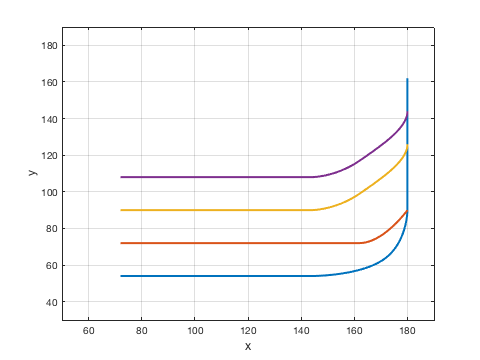
\includegraphics [width=4in]{A3_Objects_and_Path_Plus_01.eps}

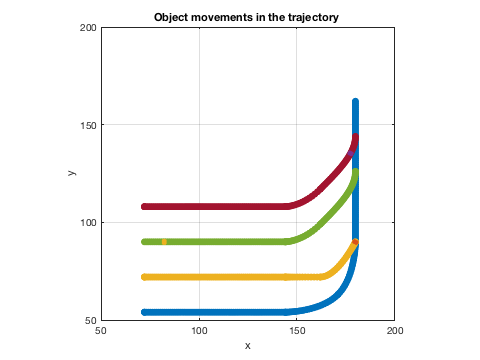
\includegraphics [width=4in]{A3_Objects_and_Path_Plus_02.eps}



\end{document}
    
